\documentclass[10pt,a4paper]{article}

\usepackage[UTF8,fontset = windows]{ctex}

\setCJKmainfont[BoldFont=黑体,ItalicFont=楷体]{等线}

\usepackage{amssymb,amsmath,amsfonts,amsthm,mathrsfs,dsfont,graphicx}

\usepackage{ifthen,indentfirst,enumerate,color,titletoc}

\usepackage{tikz}

\usepackage{multicol}

\usepackage{makecell}

\usepackage{longtable}

\usetikzlibrary{arrows,calc,intersections,patterns,decorations.pathreplacing,3d,angles}

\usepackage[bf,small,indentafter,pagestyles]{titlesec}

\usepackage[top=1in, bottom=1in,left=0.8in,right=0.8in]{geometry}

\renewcommand{\baselinestretch}{1.65}

\newtheorem{defi}{定义~}

\newtheorem{eg}{例~}

\newtheorem{ex}{~}

\newtheorem{rem}{注~}

\newtheorem{thm}{定理~}

\newtheorem{coro}{推论~}

\newtheorem{axiom}{公理~}

\newtheorem{prop}{性质~}

\newcommand{\blank}[1]{\underline{\hbox to #1pt{}}}

\newcommand{\bracket}[1]{(\hbox to #1pt{})}

\newcommand{\onech}[4]{\par\begin{tabular}{p{.9\textwidth}}

A.~#1\\

B.~#2\\

C.~#3\\

D.~#4

\end{tabular}}

\newcommand{\twoch}[4]{\par\begin{tabular}{p{.46\textwidth}p{.46\textwidth}}

A.~#1& B.~#2\\

C.~#3& D.~#4

\end{tabular}}

\newcommand{\vartwoch}[4]{\par\begin{tabular}{p{.46\textwidth}p{.46\textwidth}}

(1)~#1& (2)~#2\\

(3)~#3& (4)~#4

\end{tabular}}

\newcommand{\fourch}[4]{\par\begin{tabular}{p{.23\textwidth}p{.23\textwidth}p{.23\textwidth}p{.23\textwidth}}

A.~#1 &B.~#2& C.~#3& D.~#4

\end{tabular}}

\newcommand{\varfourch}[4]{\par\begin{tabular}{p{.23\textwidth}p{.23\textwidth}p{.23\textwidth}p{.23\textwidth}}

(1)~#1 &(2)~#2& (3)~#3& (4)~#4

\end{tabular}}

\begin{document}


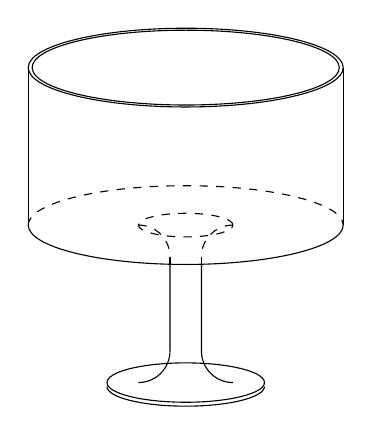
\begin{tikzpicture}
    \draw (-2,2) arc (180:-180:2 and 0.5);
    \draw (-1.95,2) arc (180:-180:1.95 and 0.475);
    \draw (-2,2) -- (-2,0) (2,2) -- (2,0);
    \draw (-2,0) arc (180:360:2 and 0.5);
    \draw [dashed] (-2,0) arc (180:0:2 and 0.5);
    \draw [dashed] (0,0) ellipse (0.6 and 0.15) (-0.6,0) arc (90:0:0.4) (0.6,0) arc (90:180:0.4);
    \draw [dashed] (-0.2,-0.4) -- (-0.2,-0.6) (0.2,-0.4) -- (0.2,-0.6);
    \draw (-0.2,-0.5) -- (-0.2, -1.6) (0.2,-0.5) -- (0.2,-1.6) 
    (-0.6,-2) arc (270:360:0.4) (0.6,-2) arc (270:180:0.4);
    \draw (-1,-2) arc (180:-180:1 and 0.25);
    \draw (-1,-2.05) arc (180:360:1 and 0.25);
\end{tikzpicture}


\end{document}